\documentclass[a4j]{jarticle}
\title{知能情報メディア実験\\ 「複数話者の同時発話音声からの個別音声の抽出」
最終レポート}
\author{情報科学類, 3年, 2クラス, 学籍番号:201311403 \ 山岡 洸瑛, Yamaoka
Kouei}
\date{2015/8/5}

%余白設定
\setlength{\topmargin}{20mm}
\addtolength{\topmargin}{-1in}
\setlength{\oddsidemargin}{20mm}
\addtolength{\oddsidemargin}{-1in}
\setlength{\evensidemargin}{15mm}
\addtolength{\evensidemargin}{-1in}
\setlength{\textwidth}{170mm}
\setlength{\textheight}{254mm}
\setlength{\headsep}{0mm}
\setlength{\headheight}{0mm}
\setlength{\topskip}{0mm}


\def\pgfsysdriver{pgfsys-dvipdfmx.def}

\usepackage{ascmac}
\usepackage{here}
\usepackage{tikz}
\usetikzlibrary{trees}
\thispagestyle{empty}
\usepackage{bm}
\usepackage{amsmath}

\usepackage{listings,jlisting}
\renewcommand{\lstlistingname}{リスト}
\lstset{
basicstyle=\ttfamily\scriptsize,
commentstyle=\textit,
classoffset=1,
keywordstyle=\bfseries,
frame=tRBl,
framesep=5pt,
showstringspaces=false,
numbers=left,
stepnumber=1,
numberstyle=\tiny,
tabsize=2
}

\begin{document}
\begin{titlepage}
\maketitle 
\thispagestyle{empty}
\end{titlepage}
\setcounter{tocdepth}{2}
\tableofcontents
\newpage

\section{はじめに}
知能情報メディア実験「複数話者の同時発話音声からの個別音声の抽出」の最終レポートとして,与えられた各課題の結果と考察をま
とめる.このレポート内において原則として,スカラーは$x$,ベクトルは太字で$\bm{x}$, 行列は大文字の太字で$\bm{X}$と表し,行列のi行j列成分を$X_{ij}$と表
すとする.その他fとmに関する行列を$\bm{X}[f,m]$とすることもある.このとき,$f=f_i, m=m_j$の場合$\bm{X}[f_i, m_j]$と表す.また単位行列を
$\bm{I}$とする.
ソースコードについては,単純な計算のみのものや,与えられた式をそのまま用いたものなどは示さない.独自に作成した
ものや,説目に必要なもののみ示す.また作成した音源についてはTAの杉本さんに確認していただいた.
\section{課題1: 瞬時混合ICAの実装}
\subsection{ステップ1}
2つの音声サンプルを$\bm{x_1}, \bm{x_2}$とし,式(1)の混合行列を用いて(2)の式で混合した.行列の形から1行2列成
分と2行1列成分の絶対値が小さいため,出力$\bm{y_1}, \bm{y_2}$について,$\bm{y_1}$
は$\bm{x_1}$の,$\bm{y_2}$は$\bm{x_2}$の音声が他方に比べて振幅が大きくなることが予想される.
\subsubsection{結果}
作成した混合を再生すると,確かに混合されていた.また,予想通り$\bm{y_1}$においては$\bm{x_1}$の音が$\bm{x_2}$よりも大きく
聞こえ,$\bm{y_2}$についても$\bm{x_2}$の方が大きく聞こえた.混合の結果を図\ref{k1s1}に示す.左側がサンプル音源,右側が混合した音声である.こ
の図からも$\bm{y_1}$は$\bm{x_1}$の,$\bm{y_2}$は$\bm{x_2}$の影響が大きいことが読み取れる.
\subsubsection{考察}
結果より,音声をベクトル化した数値で扱うことができるという事がわかった.また,音声ベクトルに対して演算を行うことが可能と
いう事もわかった.使用した混合行列の値を式(3)のように変更して混合したところ,予想通り$\bm{y_1}$では$\bm{x_2}$の,
$\bm{y_2}$では$\bm{x_1}$の音が大きくなった.これより,瞬時混合は式(4)のように単純な線形結合で表され,かつ各々の係数によっ
て音声の大きさが決まるという事が確認できた.これは音源の数が増えても$\bm{H}$のサイズが変わるだけであり,本質的には変わらないと言える.
\begin{eqnarray}
\bm{H} &=& \left(
 \begin{array}{cc}
  0.9 & 0.4\\
  -0.3 & 1
 \end{array}
\right) \\
% 式(2)
\left(
\begin{array}{c}
 \bm{y_1}\\
\bm{y_2}
\end{array}
\right)
&=& \bm{H} * 
\left(
\begin{array}{c}
 \bm{x_1}\\
 \bm{x_2}
\end{array}
\right)\\
% 式(3)
\bm{H} &=& \left(
 \begin{array}{cc}
  0.1 & 0.9\\
  0.9 & 0.1
 \end{array}
\right) \\
% 式(4)
&&
\begin{cases}
 \bm{y_1} = H_{11} * \bm{x_1} +  H_{12} * \bm{x_2} &  \\
 \bm{y_2} = H_{21} * \bm{x_1} +  H_{22} * \bm{x_2} &
\end{cases}
\end{eqnarray}

\begin{figure}[htb]
 \begin{center}
  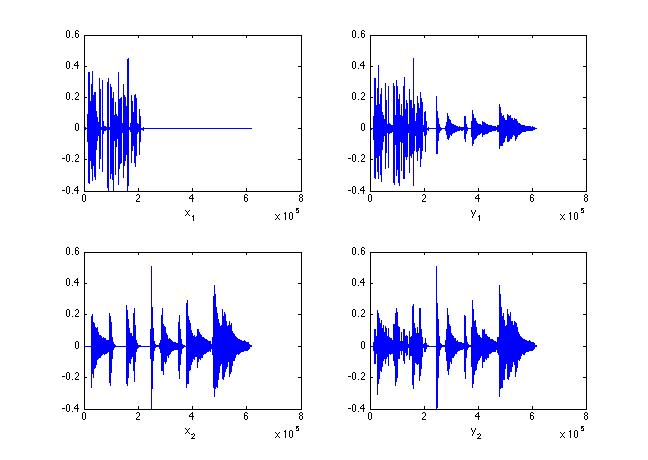
\includegraphics[width=9cm, clip, bb=0 0 648 460]{pic/k1s1.jpg}
  \caption{瞬時混合による混合}
  \label{k1s1}
 \end{center}
\end{figure}

\subsection{ステップ2}
混合行列$\bm{H}$の逆行列を用いて分離信号を作成し,それが元の音源と一致することを確認する.分離は混合音声$\bm{y_1}, \bm{y_2}$を
用いて式(5)のように行った.分離した音声を$\bm{s_1}, \bm{s_2}$とした.
\subsubsection{結果}
実際に分離を行い,元の音源と一致することが確認しできた.分離した音声をプロットしたものを図\ref{k1s2}に示す.この図が図\ref{k1s1}の右側とほぼ
一致することから視覚的にも分離できていることが確認できる.しかし同時に僅かに変わっている部分があることから知覚できない程度の誤差が生じてしまっ
ていることも読み取れる.
\subsubsection{考察}
この実験より,行列によって混合された音源は,その逆行列によって分離できるという事が確認できた.これより,混合行列が不明で
あってもその逆行列の近似的な値がわかれば分離できると予想される.生じる誤差は知覚できない程度のものなので無視してよいと言える.この誤差は
計算機で計算しているために生じる丸め誤差などの影響だと思われる.

\begin{eqnarray}
% 式(5)
 \left(
\begin{array}{c}
 \bm{s_1}\\
\bm{s_2}
\end{array}
\right)
&=& \bm{H^{-1}} * 
\left(
\begin{array}{c}
 \bm{y_1}\\
 \bm{y_2}
\end{array}
\right)
\end{eqnarray}

\begin{figure}[htb]
 \begin{center}
  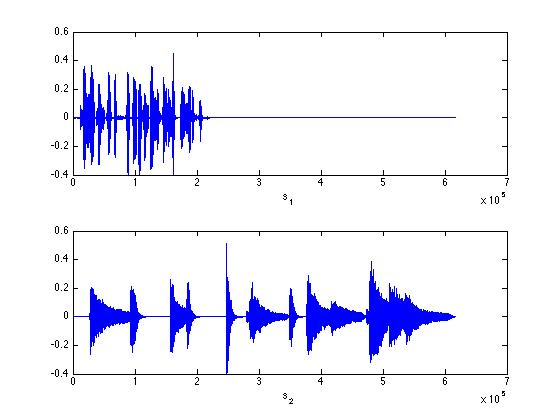
\includegraphics[width=8cm, clip, bb=0 0 560 460]{pic/k1s2.jpg}
  \caption{逆行列計算による分離}
  \label{k1s2}
 \end{center}
\end{figure}

\subsection{ステップ3}
瞬時混合ICAを用いて分離行列$\bm{W}$を学習する.インフォマックスという手法を用いて,式(6)と式(7)のような勾配法の更新を繰
り返すことによって学習する.ここで活性関数としては式(8)を用いた.
音源が2つの場合,$\bm{I}$は$2*2, i=1,2$であり,Nは音源のフレーム数である.$\bm{W}$の初期値は式(9)とし,ステップサイズ$\mu = 0.1$, 活性関数で用いる
適当な正の値$\gamma = 0.5$とした.
\subsubsection{結果}
学習した結果推定された分離行列$\bm{W}$を得た.確認のため$\bm{W} * \bm{H}$を計算したところ,1行2列成分と2行1列成分が共に0に
近くなったため,近似的な値は求まっていると言える.ただし1行1列成分,2行2列成分が大きく,単位行列からは大きく離れていた,
また,学習は勾配法で行ったため,収束条件を$\bm{W}$のすべての要素に
ついて更新前の値と更新後の値の差の絶対値が$10^{-4}$以下となること,とし反復計算を行った結果,今回のパラメータの場合179回
の反復で終了した.
\subsubsection{考察}
インフォマックスという手法を用いると分離行列が求まることが確認できた.この分離行列で実際に分離できるのかどうかはわからな
いが,結果で確認したように正しい逆行列の近似にはなっているようなので,分離できることが期待される.ただし,単位行列に近づ
かなかったことや,$\bm{W}$の要素が非常に大きいことから,元の音源よりも音量が大きくなっていると予想され,これがスケーリング
の問題であると言える.

\begin{eqnarray}
% 式(6)
 \left(
\begin{array}{c}
 \bm{y_1}\\
\bm{y_2}
\end{array}
\right)
&=& \bm{W} * 
\left(
\begin{array}{c}
 \bm{x_1}\\
 \bm{x_2}
\end{array}
\right) \\
 % 式(7)
 \bm{W} &\leftarrow & \bm{W} + \mu \left(\bm{I} - \frac{1}{N}\sum_{n=0}^{N-1}\psi (\bm{y_i}[n])\bm{y_i}[n]^t \right)\bm{W} \\
 % 式(8)
 \psi (\bm{x}) &=& \bigl(tanh\left(\gamma x_1\right), \cdots , tanh\left(\gamma x_i\right) \bigr)^t \\
 % 式(9)
\bm{W} &=& \left(
 \begin{array}{cc}
  0.3 & 0.7\\
  0.5 & 1
 \end{array}
\right)
\end{eqnarray}

\subsection{ステップ4}
ステップ1で作成した混合音声と,ステップ3で作成した分離行列を用いて実際に分離を行った.この時スケーリング解決を行った.ま
た分離性能を上げるために数回分離行列学習時のパラメータを調整した.スケーリング解決及び分離は式(10)で行った.$\bm{y_i}[n],
\bm{W}$はステップ3で得た値で,$\bm{Z}[n]$はスケーリング解決を行った分離信号である. diag()は引数を対角要素とする対角行列
を表す.
\subsubsection{結果}
分離し,スケーリング解決を行った音声を聞くと元の音源と全く同じように聞こえた.サンプル音源1の裏でサンプル音源2が少し聞こ
える,などという事はなく,完全に分離されていた.分離した音声をプロットし,図\ref{k1s4}に示す.この図からも分離していることが分かる.
スケーリングの解決もできているようで,音源1の方はほぼ完璧である.しかし,音源2の方は分離できているものの振幅が小さくなってしまっている.
\subsubsection{考察}
ステップ3で考察したように分離行列を推定することで分離することができた.パラメータの
調整は必要だが,瞬時混合の場合,正確な逆行列でなくても,非常に綺麗に分離できるといえる.スケーリングに問題は残っているが,実際に音を聞くと気
になるほどの違いはわからないため,大きな問題にはならないと言える.ここまでの計算は音源の数を2つと
して行なってきたが,音源の数が変わったとしても同じように計算できることは使用した計算式からわかる.これより瞬時混合ならば,
混合音声を分離することができると言える.

\begin{eqnarray}
 % 式(10)
 \bm{Z}[n] = \bm{W}^{-1} * diag(\bm{y_i}[n])
\end{eqnarray}

\begin{figure}[htb]
 \begin{center}
  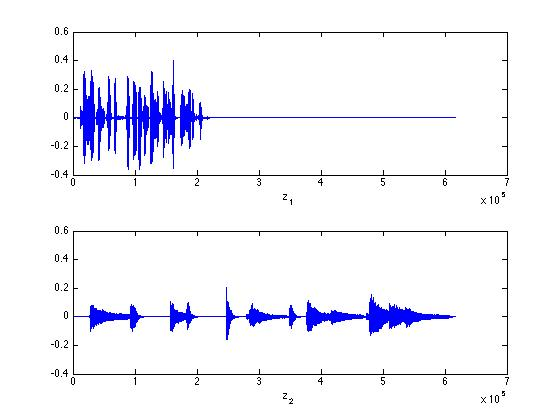
\includegraphics[width=10cm, clip, bb=0 0 560 420]{pic/k1s4.jpg}
  \caption{インフォマックスによる分離}
  \label{k1s4}
 \end{center}
\end{figure}

\subsection{ステップ5}
混合行列が与えられていない未知の瞬時混合波形に対してICAを行い音源分離を行え,という課題であったが未知の瞬時混合音声が取
得出来なかったため,混合行列$\bm{H}$の値を変えて混合音声を作成し,$\bm{H}$が未知であるとして音源分離を行った.混合行列を作成し
た翌週に分離を行うことで混合行列を未知であるとした.実際に混合行列の値は覚えていなかったため,未知であったとしても良いと
考える.
\subsubsection{結果}
ステップ4同様に分離できた.しかしステップ4と違い混合行列の情報がないとしたためパラメータの調節に時間がかかってしまった.
これは混合行列が未知であるため,分離行列との積を求めることで確認する,という方法がとれなかったため,目安がなかったことが原因であ
る.時間がかかってしまったものの分離できたためステップ4の考察で述べたように瞬時混合音声であれば分離できると言える.

\section{課題2-1: 畳み込み混合の分析}
\subsection{0.}
課題2-1で使用する畳み込み信号を自分で作成するという追加課題を行った.2音
源2マイク環境下での畳み込みを行った.インパルス応答は与えられたものを使
い,音源には課題1で使用したサンプル音源をそのまま使用した.\\ \ \ \ 
音源の長さを$N$, インパルス応答の長さを$R$として$K = N + R -1$とする.まず畳み込みを周波数領域で行うために音源とインパル
ス応答を離散フーリエ変換(以下DFTとする)する.DFTの方法としては高速フーリエ変換(以下FFTとする)を用いる.音源1,2をK点FFTした
ものを$s_1, s_2$, 音源iからマイクjへのインパルス応答をK点FFTしたものを$imp_{ij}$とする.また周波数領域でのインデックスをfと
すると,畳み込みは式(11)で表される.畳み込み混合信号を$x_i$として,$x_i$を逆フーリエ変換(以下iFFTとする)することで時間領
域の畳み込み混合信号を得る.
\subsubsection{結果}
畳み込み混合信号を得た.実際に聞いてみると音声に少しディレイがかかっているように聞こえ,畳み込みに成功していることが確認
できた.畳み込みに使用したインパルス応答を図\ref{ex2}に示す.ほとんど同じに見えるがよく見ると音源1からの第1インパルスの方が音源2からの第1イ
ンパルスよりも大きなどの違いがある.また,畳み込み混合信号を図\ref{ex1}に示す.左が元の音源で,右が畳み込み混合信号である.畳込めているのか
どうかはよく読み取れないが,振幅が$\frac{1}{10}$程度になっていることが分かる.これはインパルス応答の振幅が小さいことが原因だと思われる.これ
よりインパルス応答が反映されていると言えるため,畳み込みに成功していると言える.
\subsubsection{考察}
周波数領域における畳み込みを実装したところ非常に高速に動くことが確認できた.時間領域の畳み込みをMATLAB関数のconv()で行っ
たところメモリが足りずに計算出来なかったことから,周波数領域での畳み込みの威力が分かる.またK点FFTをする理由は,畳み込み
によって$R-1$だけ音声が伸びるからである.これは実際に短い信号で畳み込みを行なってみると確認できる.以上より以降の課題で
使用する畳み込み混合信号が作成できた.

\begin{eqnarray}
% 式(11)
\left(
 \begin{array}{cc}
  \bm{x_1}[f]\\
  \bm{x_2}[f]
 \end{array}
\right)
=
\left(
 \begin{array}{cc}
  imp11[f] & imp21[f]\\
  imp12[f] & imp22[f]
 \end{array}
\right)
*
\left(
 \begin{array}{cc}
  \bm{s_1}[f]\\
  \bm{s_2}[f]
 \end{array}
\right)
\end{eqnarray}

\begin{figure}[htb]
 \begin{center}
  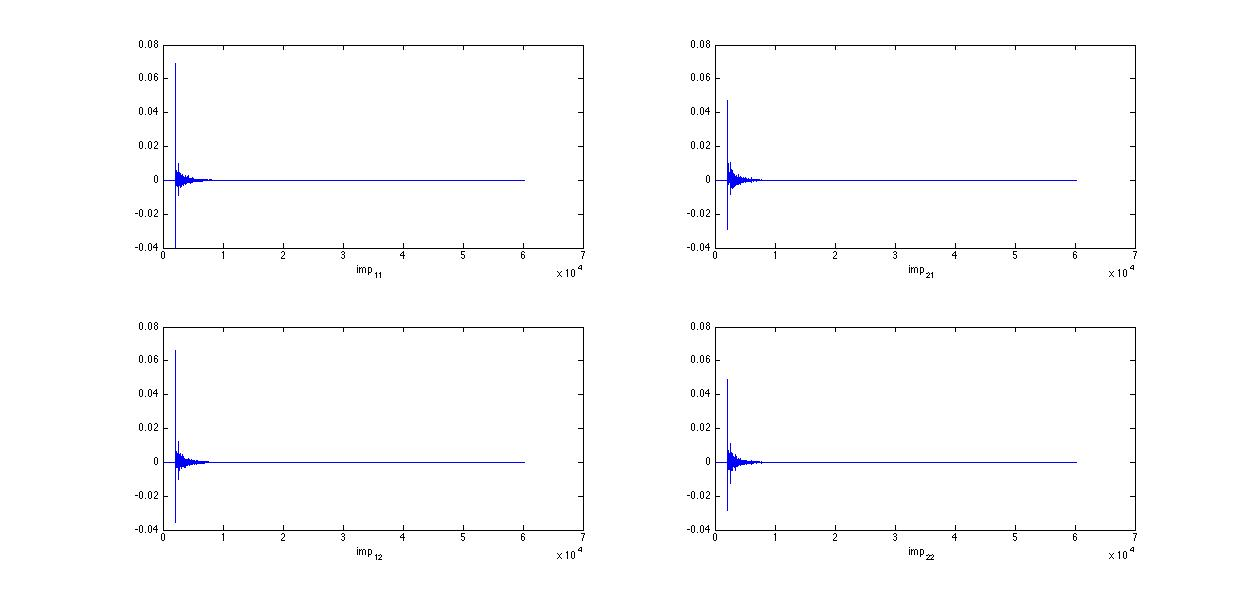
\includegraphics[width=13cm, clip, bb=0 0 1254 595]{pic/ex2.jpg}
  \caption{インパルス応答}
  \label{ex2}
 \end{center}
\end{figure}

\newpage
\begin{figure}[htb]
 \begin{center}
  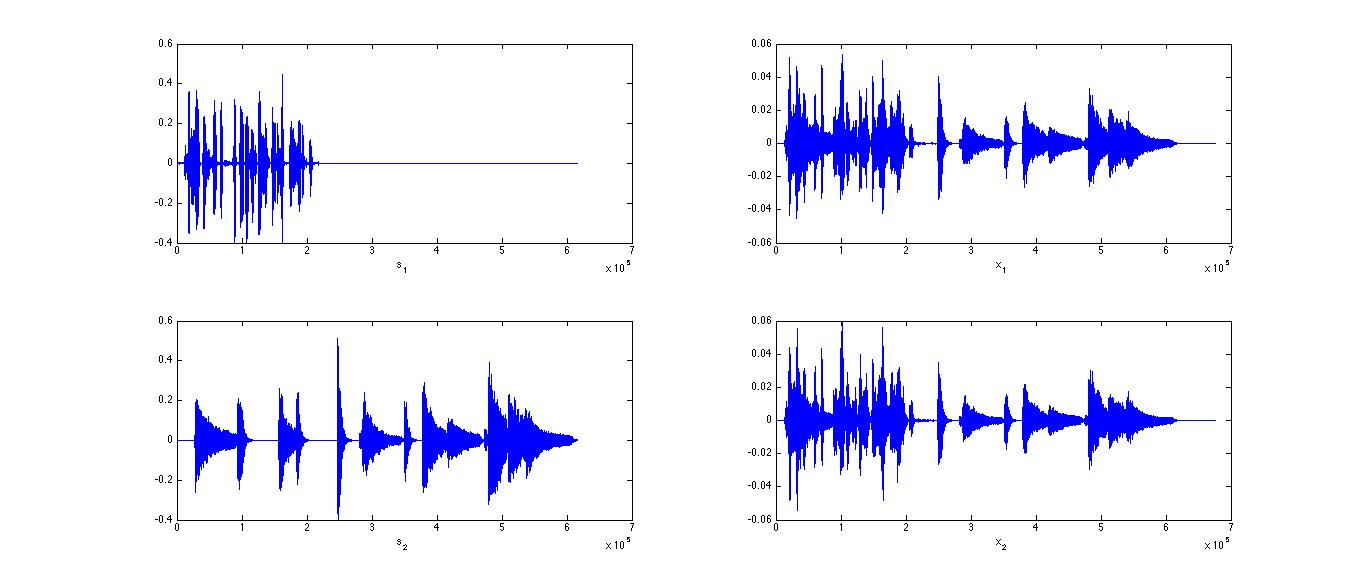
\includegraphics[width=10cm, clip, bb=0 0 1360 584]{pic/ex1.jpg}
  \caption{畳み込み混合信号}
  \label{ex1}
 \end{center}
\end{figure}

\subsection{1.}
作成した畳み込み混合信号を短時間フーリエ変換(以下STFTとする)を用いて分析する.また逆STFT(以下iSTFTとする)によって元の波
形に戻ることを確認する.
\subsubsection{実装}
フレーム長p, フレームシフトを$ol = p * \frac{1}{o}$, 総フレーム数をal, 窓関数を$\bm{w}$とする.これらを用いてpフレーム
分$\bm{w}$をかけて取り出しFFT, $ol$だけずらして同様の計算を行う.これを繰り返すことでSTFTが実装できる.iSTFTでは切り出した
フレームをiFFTして加算,olだけずらして同様の計算を行うことで実装できる.しかし,STFTの時にフレームシフトや窓関数によって
オーバーラップが生まれてしまい,その場合このままではiSTFTは正しく行えていない.例えば$ol = \frac{1}{2}$で窓関数がハミン
グ窓の場合,オーバーラップはなくこのままで良いが,窓関数が箱形窓の場合,オーバーラップは2となり,前後$\frac{p}{2}$以外は
振幅が2倍になってしまう.これを解決するためにカウント用配列を用意する.これは切り出した回数をカウントする配列で,信号の
第kインデックスをn回切り出した,という情報を格納する.iSTFT時にこの配列を用いて割ることでオーバーラップ問題を解決できる.
これに関する図を図\ref{countX}に示した.以上よりSTFT,iSTFTが実装できた.ソースコードをリスト\ref{stft.m}, \ref{istft.m}に示
す.ただし,XはSTFTした信号,YはiSTFTした信号で,countがカウント用配列である.なお,MATLABの都合上ifft()を用いてもごく小
さな値が虚数として残ってしまうことがあるため,real()関数を用いて虚数を消してある.

\subsubsection{結果}
STFTを行いiSTFTによって元の音源に戻ることが確認できた.音源信号をプロットした図を図\ref{stftistft}に示す.左側が元の音源
$s_1,s_2$で右側がSTFT,iSTFTした音源である.これより左右の信号がほぼ一致していることから,視覚的にも成功していることが確
認できた.
\subsubsection{考察}
図\ref{stftistft}の左右を見比べると僅かに異なっている部分が稀にある.これは計算機で計算しているために丸め誤差などの僅か
な誤差が生じた結果だと考えられる.左右の音源を聞いてみると,その差は知覚出来なかったため,この程度の誤差であれば無視して
も構わないと言える.また今回の実装でSTFT,iSTFTをそれぞれ関数化したため,今後STFT分析は関数1つで行えるようになった.

\newpage
\begin{figure}[htb]
 \begin{center}
  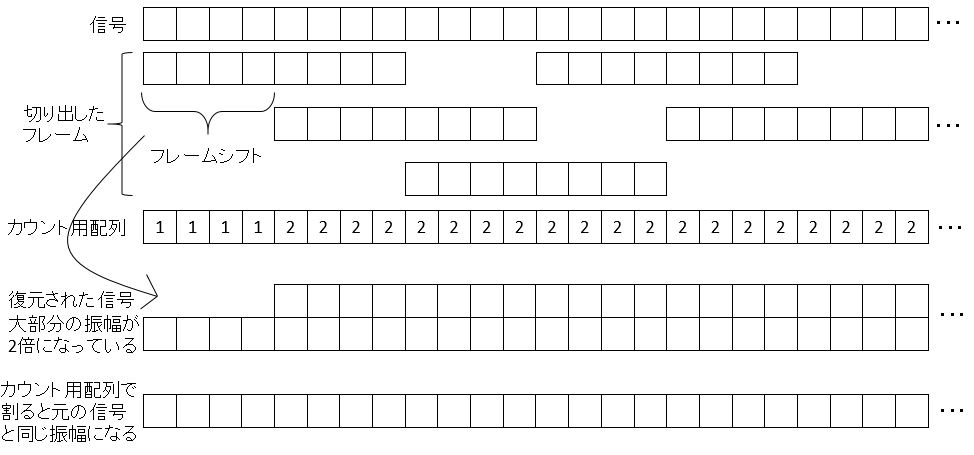
\includegraphics[width=20cm, clip, bb=-250 0 974 455]{pic/countX.jpg}
  \caption{オーバーラップ問題の解決}
  \label{countX}
 \end{center}
\end{figure}

\begin{figure}[htb]
 \begin{center}
  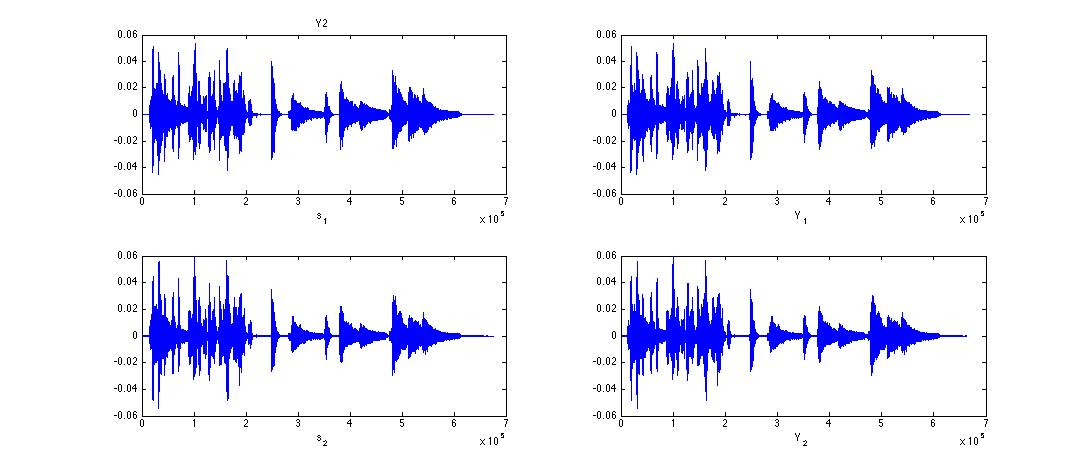
\includegraphics[width=10cm, clip, bb=0 0 1089 467]{pic/stft.jpg}
  \caption{元の音源とSTFT,iSTFT後の音源}
  \label{stftistft}
 \end{center}
\end{figure}

\begin{lstlisting}[caption=stft.m, xleftmargin=1cm, label=stft.m]
for k = 1:al
    % 窓をかけ、fft
    X(k,:) = s(1 + ol*(k-1) : p + ol*(k-1)) .* w';
    X(k,:) = fft(X(k,:));
    % 今のカウント用配列のインデックスに1加算
    count(1 + ol*(k-1) : p + ol*(k-1)) = count(1 + ol*(k-1) : p + ol*(k-1)) + 1;
end
\end{lstlisting}
\begin{lstlisting}[caption=istft.m, xleftmargin=1cm, label=istft.m]
for k = 1:al
    % ifftし窓をとる
    Y(1 + ol*(k-1) : ol*(k-1) + p) = Y(1 + ol*(k-1) : ol*(k-1) + p) + real(ifft(X(k,:))) ./ w';
end
Y = Y ./ count;
\end{lstlisting}

\subsection{2.}
与えられたインパルス応答をDFTし周波数毎の分離行列を作成する.またSTFTした混合信号を分離行列を用いて分離し,それをiSTFTす
ることで時間領域の分離信号を得る.各変数は1. と同じとし,サンプル音源1,2をSTFTしたものを$\bm{X_1}, \bm{X_2}$とする.ただしi行に第iフレームが格
納されている.また,音源iからマイクjへのインパルス応答をp点FFTしたものを$imp_{ij}$とする.分離した信号を$\bm{X_i}$と同じ
サイズの行列$\bm{Y_1}, \bm{Y_2}$に格納すると式(12)で分離することができる.ただし周波数領域のインデックスはfで表している.
計算した$\bm{Y_i}$をiSTFTすることで時間領域の分離信号を得ることができる.STFT, iSTFTは1. で作成した関数を用いるが,iSTFT
において1部変更を加えた.STFTした信号に分離行列をかけているため窓関数で割る必要がなくなったので,割らないように変更をし
た.
\subsubsection{結果}
分離に成功した. プロットした図を図\ref{k212}に示す.これより分離されていることが視覚的にも確認できる.しかし本来無音であ
るべき時間であっても僅かに振幅が存在することも確認できる.これは分離の過程で生じてしまったノイズである.これは分離した音
声を聞いても聞き取れる程度には大きく.無視することはできない.
\subsubsection{考察}
時間周波数領域での分離に成功したため,ノイズを考慮しなければ今後DFTの代わりにSTFTを使うことができる.問題のノイズが生じ
た理由について考察する.フーリエ変換は切り出した範囲が周期関数であることを仮定して計算しているため,実装したSTFTにおいて
は窓関数をかけることによってフレームの両端が綺麗につながるようにしている.しかし,切り出したフレームは実際には周期関数で
はなく,そのの続きは今のフレームとは異なる信号であるため,周期関数を仮定してDFTすると実際とは異なる周波数領域の情報が得
られてしまう.これを各フレームについて行なっているためすべてのフレームについてこのことが言える.STFT分析した信号をそのま
まiSTFTするのであれば各フレーム毎にFFTしiFFTしただけなので一致する.しかし,今回はSTFT分析した信号に分離行列をかける
という演算を行なっているため,誤差が生じたまま分離を行なっていることになる.そのため分離信号には誤差があり,それをiSTFT
しても本来の時間領域の分離信号は得られず,誤差,つまりノイズがのった信号が得られてしまう.これが理由であると考えられる.
\\\ \ \ これを解決する方法は考えつかなかった.この問題は各フレーム毎の誤差が原因であるため,フレーム長を長くすればするほ
どノイズは減少すると予想される.実際にフレーム長を長くして実行した結果を図\ref{k212long}に示す.外形自体が変わってしまっ
ている部分があるが,ノイズ部分は減少していることが読み取れる.音声のノイズも減少していると感じた.これより解決はできてい
ないが軽減はできたと言える.しかしSTFTには不確定性原理があり,フレーム長を長くすると周波数分解能は良いが時間分解能は低く
なってしまう.フレーム数を最大にすればこの問題は最も軽減されるが,それはDFTであり,STFTする意味がなくなっ
てしまう.これらよりこの問題の根本的な解決方法が見つからなかった.

\begin{eqnarray}
 % 式(12)
 \left(
 \begin{array}{cc}
  \bm{Y_1}[f]\\
  \bm{Y_2}[f]
 \end{array}
\right)
=
\left(
 \begin{array}{cc}
  imp_{11} & imp_{21}\\
  imp_{12} & imp_{22}
 \end{array}
\right)^{-1}
*
\left(
 \begin{array}{cc}
  \bm{X_1}[f]\\
  \bm{X_2}[f]
 \end{array}
\right)
\end{eqnarray}

\begin{figure}[htb]
 \begin{center}
  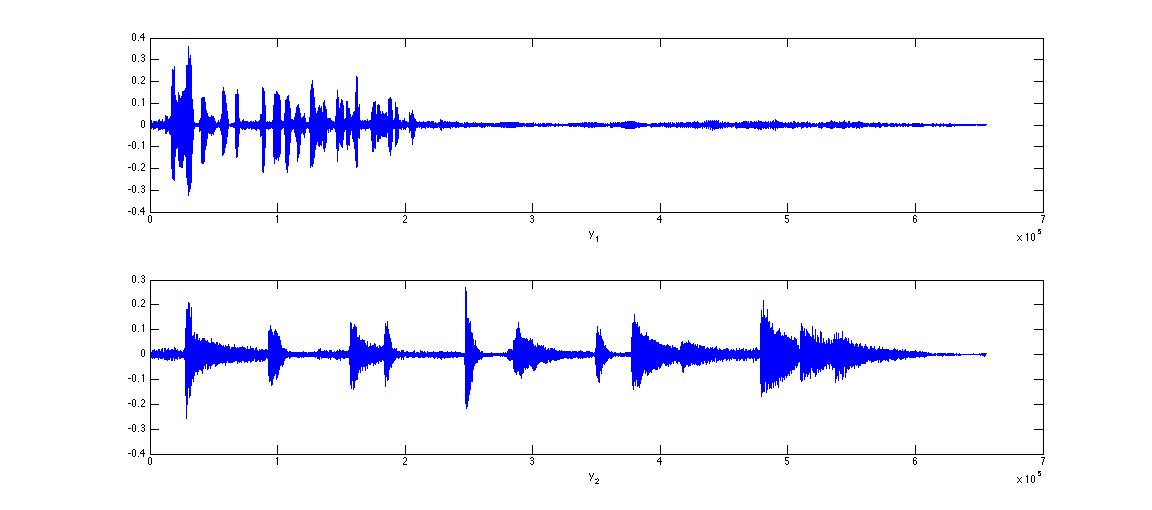
\includegraphics[width=10cm, clip, bb=0 0 1152 510]{pic/k212.jpg}
  \caption{時間領域の分離信号}
  \label{k212}
 \end{center}
\end{figure}

\begin{figure}[htb]
 \begin{center}
  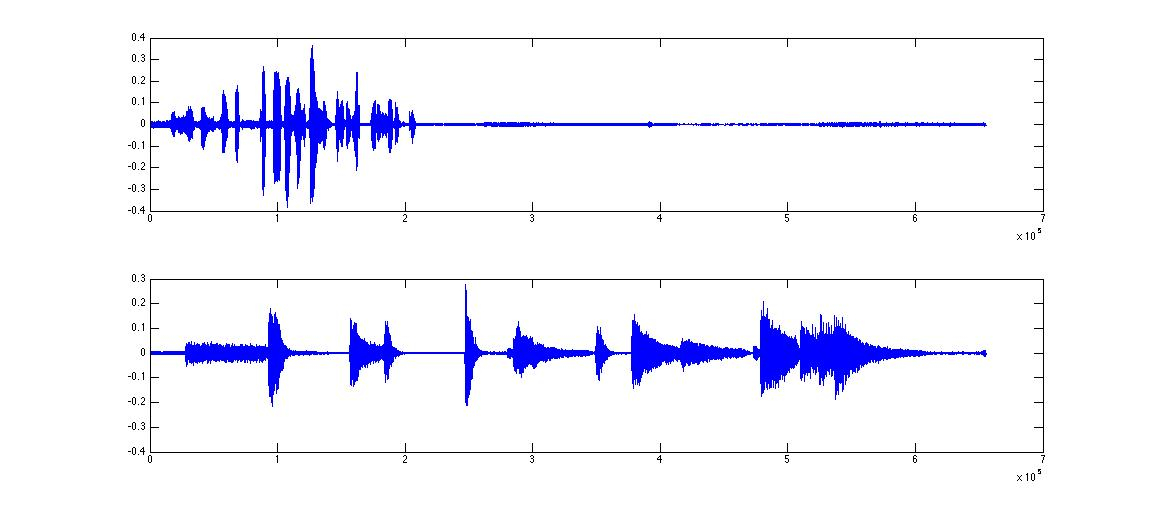
\includegraphics[width=10cm, clip, bb=0 0 1152 508]{pic/k212long.jpg}
  \caption{フレーム長を4倍にした場合}
  \label{k212long}
 \end{center}
\end{figure}

\section{課題2-2: IVAによる音源分離}
\subsection{1.}
IVAを実装し分離を行う.最大周波数を$\frac{L}{2}$とする.分離行列$\bm{W}$の学習には課題1ステップ3と同様にインフォマックスを用いる.その時の分離信号
$\bm{Y_i}$の更新は式(13)であり,勾配法の更新は式(14)である.ただしこのときの活性関数は式(15)である.活性関数で使用してい
る$\bm{normY_i}[m]$は式(16)で計算される.またスケーリングの解決は式(17)で行う.ここで$\bm{X_i}$, $\bm{Y_i}$は第i音源の時間周波数領域表現
で,周波数インデックスf, 第mフレームについて$\bm{X_i}[f,m]$などと表す.音源数が増えた場合も同様の式で計算できる.

\begin{eqnarray}
% 式(13)
\left(
 \begin{array}{cc}
  \bm{Y_1}[f,m]\\
  \bm{Y_2}[f,m]
 \end{array}
\right)
&=&
\bm{W} * 
\left(
 \begin{array}{cc}
  \bm{X_1}[f,m]\\
  \bm{X_2}[f,m]
 \end{array}
\right) \\
% 式(14)
\bm{W}[f] &\leftarrow & \bm{W}[f] + \mu \left(\bm{I} - \frac{1}{M}\sum_{m=0}^{M}\psi (\bm{Y_i}[f,m])\bm{Y_i}[f,m]^H
					\right)\bm{W}[f] \\
% 式(15)
\psi(\bm{X}[f,m]) &=& \gamma \left(\frac{Y_1[f,m]}{||normY_1[m]||_2}, \cdots ,
			      \frac{Y_J[f,m]}{||normY_J[m]||_2}\right)^t \\
% 式(16)
||normY_j[m]||_2 &=& \sqrt{\sum_{f=0}^{\frac{L}{2}} |\bm{Y_j}[f,m]|^2} \\
% 式(17)
\bm{Z} &=& \bm{W}[f]^{-1} * diag([\bm{Y_1}[f,m], \bm{Y_2}[f,m]])
\end{eqnarray}

\subsubsection{実装}
式(14)〜式(17)を実装する.しかしこのまま実装するとf,mについてループ計算が必要になるためfor文を多用することになり計算時間
が非常に長くなってしまう.そのため式変形とMATLAB関数を利用して計算速度を速くする.\\\ \ \ 
まず式(13)については音源毎にf,mについての2重ループを計算することになるが,MATLAB関数を使うことで複数の音源を同時にかつf
に関するループをなくして計算することができる.つまり音源数$* f * m$回の計算をm回の計算まで減らすことができる.まず
$\bm{X_i}, \bm{Y_i}$について,行がm,列がfとなっているが,これを2行m列fページの3次元配列に変更し,i行目に$\bm{X_i},
\bm{Y_i}$を格納する.この3次元配列を新たに$\bm{X}, \bm{Y}$とする.また$\bm{W}$を2行2列fページの3次元配列とする.
これを第fページについて式に表すと式(18)となる.この行列計算はこのままだと実行できない.$\bm{W}[f]$を対角要素とする対角行列
を用意し,$\bm{X}$を転置することで計算はできるが,メモリを大量に消費するため,ここはfor文を使うことにする.第m列に着目す
ると式(19)となり,for文で実装できる.

\begin{eqnarray}
% 式(18)
\left(
 \begin{array}{ccc}
  Y_1[f,1] & \cdots & Y_1[f,M]\\
  Y_2[f,1] & \cdots & Y_2[f,M]
 \end{array}
\right) &=& 
\left(
\begin{array}{cc}
 W_{11}[f]&W_{12}[f] \\
 W_{21}[f]&W_{22}[f]
\end{array}
\right) * 
\left(
 \begin{array}{ccc}
  X_1[f,1] & \cdots & X_1[f,M]\\
  X_2[f,1] & \cdots & X_2[f,M]
 \end{array}
\right) \\
% 式(19)
\left(
 \begin{array}{ccc}
  Y_1[f,m]\\
  Y_2[f,m]
 \end{array}
\right) &=& 
\left(
\begin{array}{cc}
 W_{11}[f]&W_{12}[f] \\
 W_{21}[f]&W_{22}[f]
\end{array}
\right) * 
\left(
 \begin{array}{ccc}
  X_1[f,m]\\
  X_2[f,m]
 \end{array}
\right) \\
&=&
\left(
 \begin{array}{ccc}
  W_{11}[f] * X_1[f,m] + W_{12}[f] * X_2[f,m]\\
  W_{21}[f] * X_1[f,m] + W_{22}[f] * X_2[f,m]
 \end{array}
\right) \nonumber
\end{eqnarray}

これは行列ならば簡単に計算できる式だが,3次元配列の場合MATLABでは計算することができない.そのためこの式をMATLABで計算で
きるように式変形すると式(20)となり,これは式(19)と一致する.そしてこの式は3次元配列のままMATLABで計算できる.これによっ
てfに関するfor文の撤去に成功した.sum(), .*, はMATLAB表記で,$\bm{X}^t$は転置を表す.ソースコードはリスト\ref{bunri.m}に示す.
\begin{eqnarray}
% 式(20)
&& sum \left(
\left(
 \begin{array}{ccc}
  W_{11}[f] & W_{12}[f]\\
  W_{21}[f] & W_{22}[f]
 \end{array}
\right) 
.*
\left(
 \begin{array}{ccc}
  X_1[f,m] & X_1[f,m]\\
  X_2[f,m] & X_2[f,m]
 \end{array}
\right)^t
, 2\right) \\
&=& 
sum \left(
\left(
 \begin{array}{ccc}
  W_{11}[f] * X_1[f,m] & W_{12}[f] * X_2[f,m]\\
  W_{21}[f] * X_1[f,m] & W_{22}[f] * X_2[f,m]
 \end{array}
\right) 
, 2\right) \nonumber \\
&=& 
\left(
 \begin{array}{ccc}
  W_{11}[f] * X_1[f,m] + W_{12}[f] * X_2[f,m]\\
  W_{21}[f] * X_1[f,m] + W_{22}[f] * X_2[f,m]
 \end{array}
\right) \nonumber
\end{eqnarray}

次に式(14)〜(16)について考える.まず,式(20)で計算した$\bm{Y}$からそれぞれの信号を取り出し,m行f列の$\bm{Y_1}, \bm{Y_2}$
とする.これを用いると,要素毎に2乗し,sum()を使い,sqrt()を使うことで式(21)となり,式(16)を得る.これより式(16)にはf,m
どちらのfor文もいらず,音源毎の計算をすれば良い.
 \begin{eqnarray}
% 式(21)
\left(||normY_j[1]||_2, \cdots , ||normY_j[M]||_2 \right) &=& \left(\sqrt{\sum_{f=0}^{\frac{L}{2}}
 |\bm{Y_j}[f,1]|^2}, \cdots , \sqrt{\sum_{f=0}^{\frac{L}{2}} |\bm{Y_j}[f,M]|^2} \right)  
 \end{eqnarray}
式(15),(16)を用いて式(14)を音源を同時にかつfに関するfor文のみで計算できるようにする.つまり計算回数が音源数$*f*m$回であっ
たのをf回に減らす.まず式(14)中の$\psi (\bm{Y_i}[f,m])\bm{Y_i}[f,m]^H$について式変形をする.以下の式変形において,MATLAB
関数のsum(), 複素共役をとるconj(), 内積を計算するdot()を用いる.なお以下では音源数をJとしている.

\begin{eqnarray}
 \psi (\bm{Y_i}[f,m])\bm{Y_i}[f,m]^H &=& 
\gamma \left(
\begin{array}{c}
 \frac{Y_1[f,m]}{normY_1[m]}\\
 \vdots \\
 \frac{Y_J[f,m]}{normY_J[m]}
\end{array}
\right)
\left(
 \begin{array}{ccc}
  conj(Y_1[f,m]),&\cdots, & conj(Y_J[f,m])\\
 \end{array}
\right)  \nonumber \\
&=& \gamma
\left(
\begin{array}{ccc}
 \frac{Y_1[f,m] * conj(Y_1[f,m])}{normY_1[m]}, & \cdots, & \frac{Y_1[f,m] * conj(Y_J[f,m])}{normY_1[m]}\\
 \vdots & \ddots & \vdots \\
 \frac{Y_J[f,m] * conj(Y_1[f,m])}{normY_J[m]}, & \cdots, & \frac{Y_J[f,m] * conj(Y_J[f,m])}{normY_J[m]}
\end{array}
\right) \nonumber \\
\sum_{m=1}^{M} \psi (\bm{Y_i}[f,m])\bm{Y_i}[f,m]^H &=& \gamma
\left(
\begin{array}{ccc}
 \sum_{m=1}^{M}\frac{Y_1[f,m] * conj(Y_1[f,m])}{normY_1[m]}, & \cdots, & \sum_{m=1}^{M}\frac{Y_1[f,m] * conj(Y_J[f,m])}{normY_1[m]}\\
 \vdots & \ddots & \vdots \\
 \sum_{m=1}^{M}\frac{Y_J[f,m] * conj(Y_1[f,m])}{normY_J[m]}, & \cdots, & \sum_{m=1}^{M}\frac{Y_J[f,m] * conj(Y_J[f,m])}{normY_J[m]}
\end{array}
\right) \nonumber \\
&=& \gamma
\left(
\begin{array}{ccc}
 \frac{dot\bigl(\bm{Y_1}[f],\ conj(\bm{Y_1}[f])\bigr)}{sum(\bm{normY_1})}, & \cdots, & \frac{dot\bigl(\bm{Y_1[f]},\ conj(\bm{Y_J[f]})\bigr)}{sum(\bm{normY_1})}\\
 \vdots & \ddots & \vdots \\
 \frac{dot\bigl(\bm{Y_J}[f],\ conj(\bm{Y_1}[f])\bigr)}{sum(\bm{normY_J})}, & \cdots, & \frac{dot\bigl(\bm{Y_J[f]},\ conj(\bm{Y_J[f]})\bigr)}{sum(\bm{normY_J})}
\end{array}
\right) 
\end{eqnarray}
式(22)において$dot\bigl(\bm{Y_j}[f],\ conj(\bm{Y_j}[f])\bigr)$は,行列$\bm{Y_j}[f,m]$の第f列を取り出したベクトル
$\bm{Y_j}[f]$とその複素共役の内積であるからスカラーであり,$sum(\bm{normY_1})$はベクトルの要素の和なのでこちらもスカラー
である.従って$J*J$の行列である.この行列を$\bm{\chi}[f]$とおくと,式(14)は以下のように表される.これを更に式変形する.
\begin{eqnarray}
 \bm{W}[f] &\leftarrow & \bm{W}[f] + \mu \left(\bm{I} - \frac{1}{M} \bm{\chi}[f] \right)\bm{W}[f] \nonumber \\
 &=& \left(\bm{I} + \mu \left(\bm{I} - \frac{1}{M} \bm{\chi}[f] \right) \right) \bm{W}[f] \nonumber
\end{eqnarray}
ここで改めて$\bm{I} + \mu \left(\bm{I} - \frac{1}{M} \bm{\chi}[f] \right)$を$\bm{\chi}[f]$とおくと,最終的に式(14)は式(23)と表
すことができる.
\begin{eqnarray}
 \bm{W}[f] \leftarrow \bm{\chi}[f] * \bm{W}[f]
\end{eqnarray}
この計算は3次元配列であるため行えないが,第i列について1列ずつ行えば,式(13)と同じ方法で実行できる.以上より全ての音源を
同時にfのループのみで実行できるようになった.ソースコードはリスト\ref{bunri.m}に示す.式(22)を計算する関数calcm.mはリスト
\ref{calcm}に示す.\\\ \ \ 
これより分離行列の学習が実装できた.これを用いると,混合信号をSTFTし分離行列を学習,学習した分離行列を用いて式(13)のよう
に分離,式(17)でスケーリング解決を行いiSTFTすることで時間領域の分離信号を得ることができる.STFT, iSTFTについては実装済み
なので省略する.

\begin{lstlisting}[caption=bunri.m, xleftmargin=1cm, label=bunri.m]
% 反復計算
for k=1:loop
    % 式(13)の計算
    for l = 1:fi
        Y(:,l,:) = sum(W .* repmat(permute(X(:,l,:),[2,1,3]), 2, 1), 2);
    end
    %Yの計算終了----------------------------------------------------
    
    % Wの更新------------------------------------------------
    % 準備
    Y1 = squeeze(Y(1,:,:)).';
    Y2 = squeeze(Y(2,:,:)).';
    % 式(16)の計算
    normY1 = sqrt(sum(abs(Y1).^2));
    normY2 = sqrt(sum(abs(Y2).^2));
    
    % X[f]の計算
    for i = 1:L2
        kai(:,:,i) = calcm(Y1(i,:), Y2(i,:), normY1, normY2, fi, mu, ganma);
    end

    % 式(23)の計算
    W(:,1,:) = sum(kai .* repmat(permute(W(:,1,:),[2,1,3]), 2,1), 2); 
    W(:,2,:) = sum(kai .* repmat(permute(W(:,2,:),[2,1,3]), 2,1), 2); 

    % Wの更新終了----------------------------------------------------
end

% 最後の式(13)の計算
for l = 1:fi
    Y(:,l,:) = sum(W .* repmat(permute(X(:,l,:),[2,1,3]), 2, 1), 2);
end
\end{lstlisting}
\begin{lstlisting}[caption=calcm.m, xleftmargin=1cm, label=calcm]
function kai = calcm(Y1, Y2, normY1, normY2, fi, mu, ganma)

ty1 = ganma * conj(Y1);
ty2 = ganma * conj(Y2);
kai = [sum((Y1.*ty1)./normY1), sum((Y1.*ty2)./normY1); ...
        sum((Y2.*ty1)./normY2), sum((Y2.*ty2)./normY2)];
kai = eye(2) + mu * (eye(2) - (1/fi) * tmpY);
\end{lstlisting}
\subsubsection{結果}
分離に成功した.$\bm{W}$の初期値はシード値509で生成した乱数とした.$\mu, \gamma$は分離精度を上げるために変更しつつ調整し
た.分離音声$\bm{Y_1}, \bm{Y_2}$をプロットした図を図\ref{picbunri}に示す.この図からわかる通り,分離には成功したが完全に分離することは出来な
かった.分離,というよりは片方の音源を強調していると言ったほうがいいかもしれない.どちらかの一方の音が大きく聞こえ,他方の音が後ろで小さく聞
こえている.課題1ステップ4のようには分離出来なかった.分離精度の向上が今後の課題と言える.

\subsubsection{考察}
まず計算回数を減らすためにした式変形によってどの程度計算速度が上がったのかを確認する.残ったfor文はfに関するものとmに関
するもの両方あるため,for文の計算速度はトレードオフの関係になってしまっている.今回はフレーム長を1024として実行した.こ
の時,式(13)は0.2秒短縮され,式(14)については6秒程度短縮された.フレーム長を長くすると式(13)は更に短縮されるが,式(14)は
長くなってしまう.これよりフレーム長にかかわらず約6秒程度の短縮になったと言える.ただし混合信号の長さが短くなると短縮される
時間も短くなる.これはf,mどちらも小さくなるためfor文自体にかかる時間が減るためである.このことから当然ではあるが,今回の短縮は混合信号が
長いほど威力を発揮すると言える.\\\ \ \
また特に式(13)などはわかりやすくするため音源数が2個の場合で式変形しているが,音源数がJ個の場合も同じ方法で実装することが
できる.これより畳み込み混合信号であっても分離行列を学習し分離できるようになった.ここまでで音源数とマイクの数が適してい
れば実際の環境下で混合音声を分離できるようになったはずである.必要な情報は話者の数とマイクの数,話者の数以上の混合信号の
みである.\\\ \ \ 

\begin{figure}[htb]
 \begin{center}
  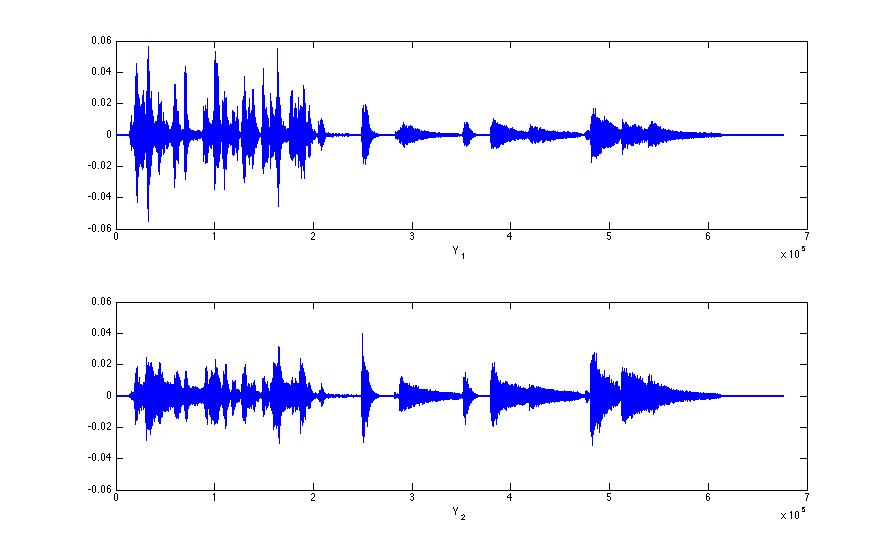
\includegraphics[width=10cm, clip, bb=0 0 892 550]{pic/samplebunri.jpg}
  \caption{分離信号}
  \label{picbunri}
 \end{center}
\end{figure}

\subsection{2.}
この課題はやらない,という事なので行わなかった.配布するという関数も配布されなかったため実装出来なかった.

\section{課題2-3: 分離性能の客観・主観評価}

\subsection{1.}
客観評価に使用する音源が配布されなかったため行わなかった.この課題もやらない,という事であった.

\subsection{2.}
実環境で録音した信号の分離を行う.録音した音声は2話者の場合と3話者の場合があり,その両方について分離を行った.分離には課
題2-2で作成したプログラムをその儘使用した.3話者の場合には同様の手法で音源数を3つに拡張したプログラムを使用した.分離し
た音源を用いて主観評価実験も行う.
\subsubsection{結果}
分離に成功した.ただし前の課題と同じくパラメータを調整したが,完全には分離できず1人が話している後ろで僅かに別の人間の話し声が残ってしまっ
た.またノイズも大きく,それほど精度が高いとは言えないものとなった.しかし1人の話し声だけが強く聞こえるため成功と言える
だろう.2話者の場合でもノイズなどが大きかったにも関わらず,3話者のばあいはそれがさらに大きくなってしまい,精度は更に悪く
なってしまった.混合信号によってはうまく分離できず,1人の声が少し大きくなったぐらいにしかならないこともあり,3話者の分離
は困難であった.例として2話者の場合と3話者の場合それぞれについて,混合信号と分離信号を図\ref{bunri2},\ref{bunri3}に示す.どちらも左側が混合
信号で右側が分離信号である.図の通り,ノイズが非常に大きくなってしまっているが,振幅が大きな位置が異なっていることから分離に成功しているこ
とが分かる.特に3話者の場合はほとんどノイズなのではないかと思うほどノイズが大きいが,こちらも大きな振幅の位置で分離されていることが読み取れ
る.これでも分離精度が最も良いと感じたものを選んでプロットしたのである.このノイズ除去は重要な課題であると言える.
\subsubsection{考察}
今回の分離でノイズが大きくなってしまった一因に元の混合信号にもノイズが乗っていたという事が挙げられる.これに関してはこち
らではどうしようもないため,改善は難しいだろう.改善方法としてバンドパスフィルタを通してみた.人間が通常会話で発する音の
周波数は300〜2000Hz程度の範囲に収まるため,それ以外の周波数をカットすることでノイズが減少するのではないか,という単純な
考えから行なってみた.しかし実際にはノイズは減少せず,理由はわからなかったがノイズが大きくなってしまうこともあった.これ
より単純なバンドパスフィルタではノイズ除去は行えないことがわかった.ノイズの特性を調べてみるとはっきりしたことはわからな
かったが,白色雑音も含まれているようで,これからも単純なフィルタでは除去できないことが分かる.\\\ \ \ 
分離精度についてもパラメータを何度も調整したにも関わらず上がらないため,この分離方法ではそれほど精度を得られないのだと思
われる.分離音声と混合音声を聞いていると,話者の声の大きさなど,個人差があるためそれによって精度が変わってくるように感じ
られた.例えば声が比較的大きい人と小さい人の2話者で分離すると,大きい人の方が分離精度が高く,小さい人の場合はそれほど高
くなくなってしまっている.これより分離は混合信号に強く左右される,と言える.高精度の分離には限界があり,高精度の混合信号
が必要なのではないだろうか.

\begin{figure}[htb]
 \begin{center}
  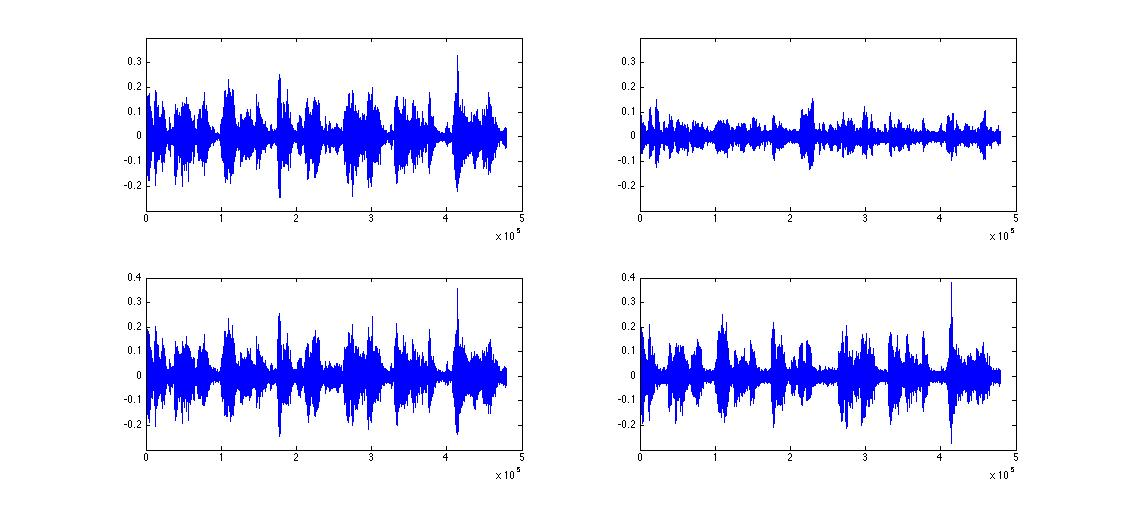
\includegraphics[width=13cm, clip, bb=0 0 1123 506]{pic/bunri2.jpg}
  \caption{2話者の場合の分離}
  \label{bunri2}
 \end{center}
\end{figure}

\newpage
\begin{figure}[htb]
 \begin{center}
  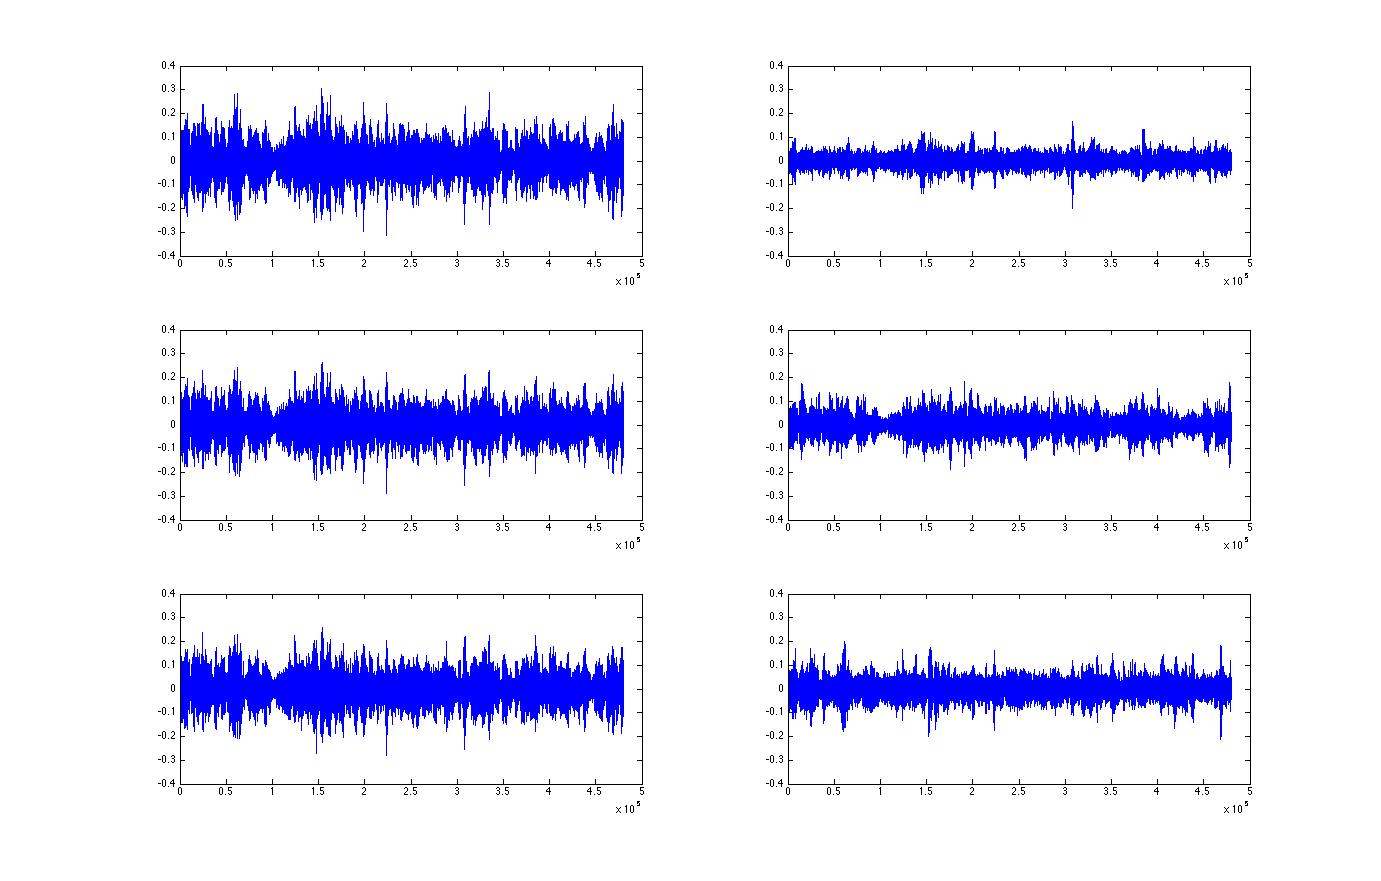
\includegraphics[width=13cm, clip, bb=0 0 1381 881]{pic/bunri3.jpg}
  \caption{3話者の場合の分離}
  \label{bunri3}
 \end{center}
\end{figure}
\subsubsection{主観評価実験}
分離した音源を用いて主観評価実験を行った.今回の実験は合計5人で行ったため,その5人の分離音声を集め,誰の音声かわからない状態でランダムに再生,
それを音質,分離という2項目について5段階評価を行った.音質は分離にかかわらず,良いかどうか,分離は音質に関わらず,分離できているかできていな
いか,が評価基準であった.結果がまだわからないため,自分の分離精度がどの程度なのかはわからないが,中には自分のよりも明らかに精度よく分離でき
ているものもあり,工夫次第でまだまだ精度をあげられることがわかった.

\section{終わりに}
この実験の結果,混合信号の分離を学ぶ過程で信号処理について理解が深まった.特に式で扱っただけのフーリエ変換を実際に行った
ことで,利用方法を学ぶことができた.また混合信号分離についての知識と技術も手に入れることができた.
分離精度の向上や,ノイズの除去など課題は多いが,この実験の目標は達成できたと言えるだろう.

\end{document}
